% =============================================================================
% EXPERIMENTS
% =============================================================================

\label{sec:experiments}

\subsection{Training Pipeline}

We follow a stacked training pipeline (Figure~\ref{fig:architecture}): Base $\rightarrow$ SFT $\rightarrow$ DPO $\rightarrow$ CITA on \texttt{Llama-3.1-8B} with PKU-SafeRLHF data (A100-40GB).

\begin{figure}[H]
\centering
\small
\setlength{\tabcolsep}{2pt}
\begin{tabular}{ccccccc}
\textit{\scriptsize Llama-3.1-8B} & & \textit{\scriptsize PKU (chosen)} & & \textit{\scriptsize PKU (pref. pairs)} & & \textit{\scriptsize + Instructions} \\[2pt]
$\downarrow$ & & $\downarrow$ & & $\downarrow$ & & $\downarrow$ \\[2pt]
\fbox{\textbf{Base}} & $\rightarrow$ & \fbox{\textbf{SFT}} & $\rightarrow$ & \fbox{\textbf{DPO}} & $\rightarrow$ & \colorbox{green!20}{\fbox{\textbf{CITA}}} \\[2pt]
& & $\downarrow$ & & $\downarrow$ & & $\downarrow$ \\[2pt]
& & $\mathcal{L}_{\text{SFT}}$ & & $\mathcal{L}_{\text{DPO}}$ & & $\mathcal{L}_{\text{CITA}} + \lambda \cdot \text{KL}$ \\
\end{tabular}
\caption{CITA training pipeline. Each stage builds on the previous checkpoint. CITA adds mandatory KL regularization for instruction-conditioned alignment.}
\label{fig:architecture}
\end{figure}

\subsection{Model Variants}

We train 4 variants to compare CITA vs DPO:

\begin{table}[H]
\centering
\small
\begin{tabular}{@{}ll@{}}
\toprule
\textbf{Model} & \textbf{Training Path} \\
\midrule
CITA\_NI & Base$\rightarrow$SFT$\rightarrow$DPO$\rightarrow$CITA \\
CITA\_I & Base$\rightarrow$SFT$\rightarrow$DPO$\rightarrow$CITA \\
DPO\_NI & Base$\rightarrow$SFT$\rightarrow$DPO \\
DPO\_I & Base$\rightarrow$SFT$\rightarrow$DPO \\
\bottomrule
\end{tabular}
\caption{Model variants. NI=NoInstruct, I=Instruct.}
\label{tab:model_variants}
\end{table}

\subsection{Evaluation Benchmarks}

We evaluate on 5 benchmarks (excluding Toxicity which uses LLM-as-judge):

\begin{table}[H]
\centering
\footnotesize
\begin{tabular}{@{}lcc@{}}
\toprule
\textbf{Benchmark} & \textbf{Test Cases} & \textbf{Variants} \\
\midrule
ISD & 3,000 & 10 types \\
TruthfulQA & 1,634 & HON/CONF \\
Cond. Safety & 1,000 & STR/PERM \\
Style Transfer & 1,000 & CON/DET \\
AQI & 2,800 & 7 axioms \\
\bottomrule
\end{tabular}
\caption{Evaluation benchmarks. All use deterministic metrics (no LLM judge).}
\label{tab:benchmarks}
\end{table}

\begin{table}[H]
\centering
\footnotesize
\begin{tabular}{@{}ll@{}}
\toprule
\textbf{Benchmark} & \textbf{Metric (Ideal)} \\
\midrule
ISD & Fidelity$\times$Shift (1.0) \\
TruthfulQA & HON$-$CONF uncert. (+) \\
Cond. Safety & $|$STR$-$PERM$|$ (1.0) \\
Style Transfer & DET/CON words ($>$4) \\
AQI & (CHI+XB)/2 (100) \\
\bottomrule
\end{tabular}
\caption{Metric formulas and ideal scores.}
\label{tab:metrics}
\end{table}

\textbf{ISD types}: Neutral, Conservative, Liberal, Regulatory, Empathetic, Safety, Educational, Concise, Professional, Creative.

\textbf{AQI axioms}: Civility, Duty, Empathy, Information, Justice, Well-being, Wisdom.

\subsection{Hyperparameter Optimization}

We use Optuna with TPE sampler (12 trials) to find optimal hyperparameters. Key finding: \textbf{CITA\_Instruct requires 50\% lower learning rate} than CITA\_NoInstruct because instruction-augmented sequences are 30--40\% longer, causing larger gradients.

\begin{table}[H]
\centering
\footnotesize
\begin{tabular}{@{}lcc@{}}
\toprule
\textbf{Hyperparameter} & \textbf{NoInstruct (T5)} & \textbf{Instruct (T7)} \\
\midrule
Learning rate & 6.83e-6 & 5.41e-6 \\
$\lambda_{\text{KL}}$ & 0.00052 & 0.00023 \\
$\beta$ (DPO temp.) & 0.119 & 0.107 \\
Weight decay & 0.0091 & 0.0109 \\
Warmup ratio & 7.5\% & 10.0\% \\
\midrule
Final margin & 6.95 & 7.52 \\
Accuracy & 89.5\% & 89.0\% \\
\bottomrule
\end{tabular}
\caption{Best hyperparameters from Optuna. T5/T7 = Trial number.}
\label{tab:hyperparams}
\end{table}

\subsection{Training Dynamics}

Figure~\ref{fig:training_cita} shows training curves from TensorBoard. CITA achieves higher reward margins than DPO with stable convergence.

\begin{figure*}[!t]
\centering
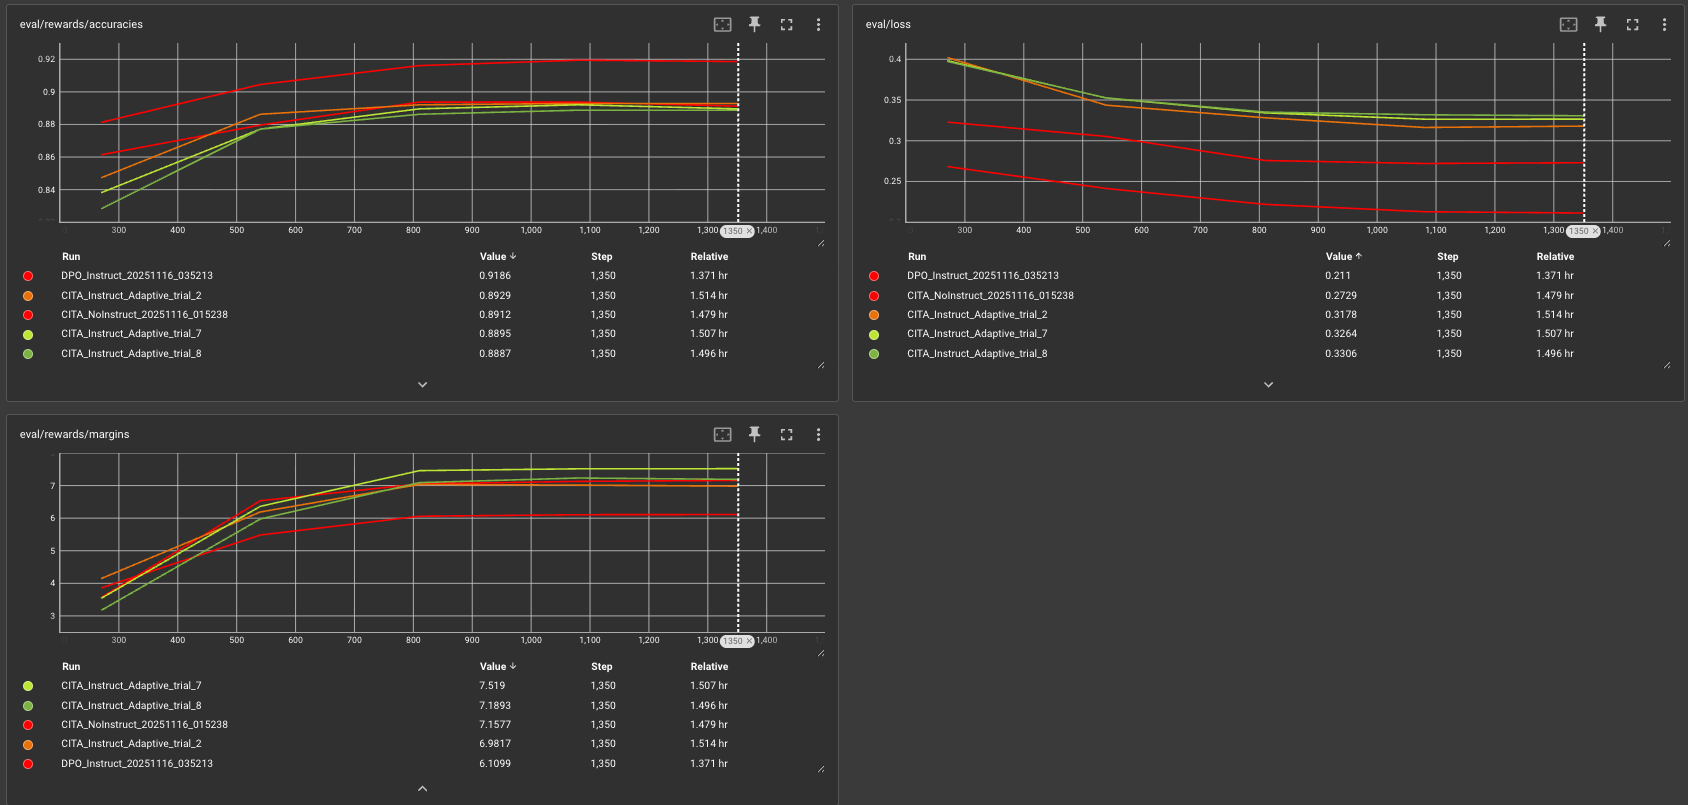
\includegraphics[width=0.85\textwidth]{figures/training/CITA_Instruct_Best3Trials_vs_DPO_Instruct_CITA_NoInstruct.png}
\caption{Training curves: Best CITA\_Instruct trials (Optuna) vs DPO\_Instruct and CITA\_NoInstruct. Top-left: accuracy, top-right: eval loss, bottom: reward margins.}
\label{fig:training_cita}
\end{figure*}

\begin{figure*}[!t]
\centering
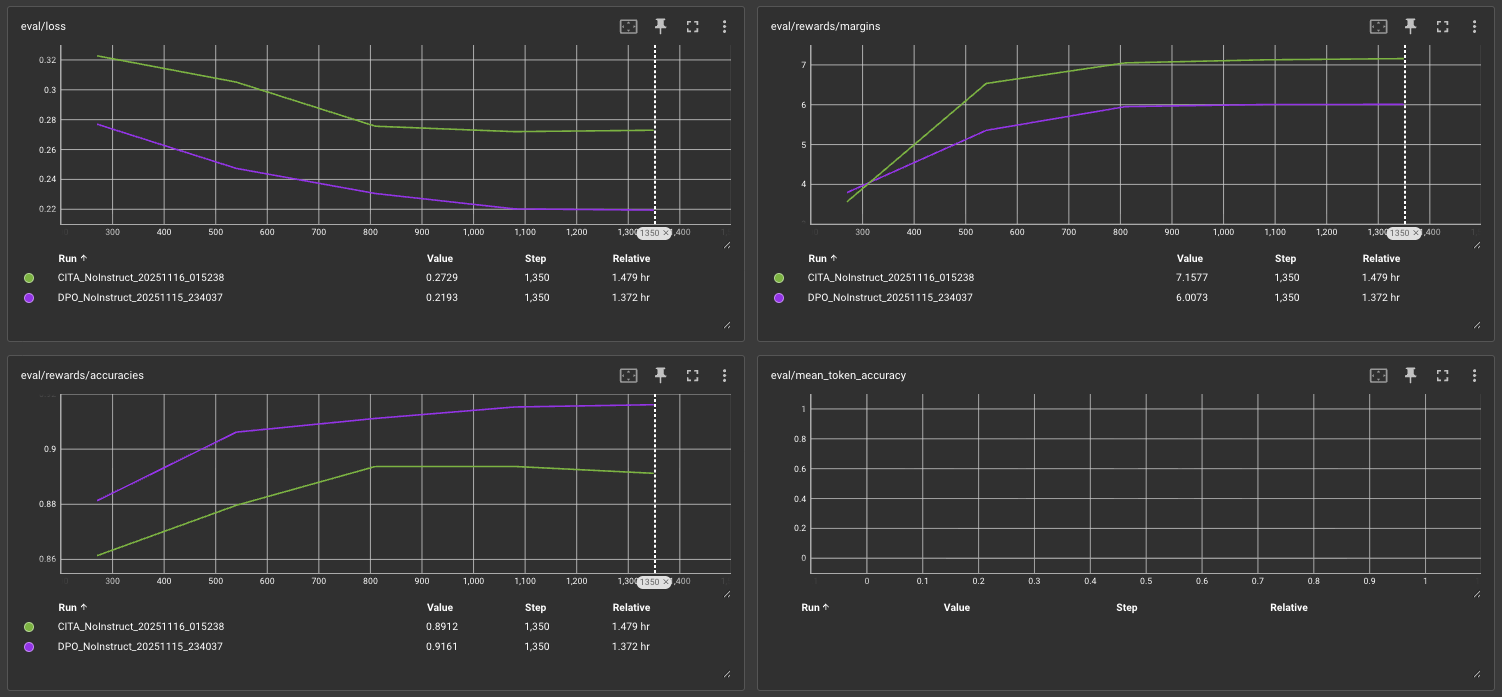
\includegraphics[width=0.85\textwidth]{figures/training/DPO_NoInstruct_vs_CITA_NoInstruct.png}
\caption{DPO vs CITA (NoInstruct): CITA achieves higher margins (7.16 vs 6.01) validating the KL-regularized objective.}
\label{fig:training_dpo_cita}
\end{figure*}
